\subsection{Flytdiagram}
\begin{flushleft}
Undersøkelse av nåværende system for transport av bil inn og ut av tilhenger, viser at det er mest hensiktsmessig å benytte seg av en rammekonstruksjon som bilen plasseres på. Rammekonstruksjonen med bilen på blir så ført videre inn i tilhengeren. Dette prinsippet er valgt å benytte videre. For å lettere få oversikt over de ulike trinnene i prosessen med å få bilen inn og ut av tilhengeren, settes det opp et flytskjema.
\end{flushleft}

\begin{figure}[H]
\begin{center}
\leavevmode
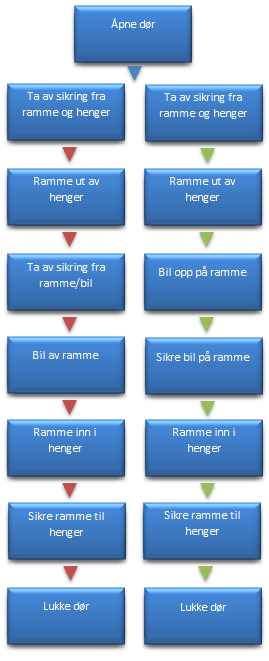
\includegraphics[width=\textwidth]{images/Bildet_3}
\end{center}
\caption{Flytdiagram}
\label{fig:flowchart}
\end{figure}

\begin{flushleft}
Øverst vises operasjonene med å ta bilen ut av tilhengeren, nederst vises stegene i prosessen med å flytte bilen inn i tilhengeren.\newpage

\subsection{Morfologisk tabell}
Basert på flytdiagrammet settes det opp en morfologisk tabell. Denne er vist nedenfor.
\end{flushleft}

\begin{table}[H]
\begin{center}
\begin{tabular}{| l | l | p{3cm} |}
\hline
\multicolumn{3}{|c|}{Morfologisk tabell} \\
\hline
\multirow{4}{*}{Flytte bil ved hjelp av} 
 & 1.1 & Plate \\
 & 1.2 & Ramme \\
 & 1.3 & Krok \\
 & 1.4 & Pute \\ \hline
\multirow{2}{*}{Inn og ut av tilhenger} 
 & 2.1 & Rulle \\
 & 2.2 & Løfte \\ \hline
\multirow{2}{*}{Drivkraft} 
 & 3.1 & Elektrisk \\
 & 3.2 & Muskelkraft \\ \hline
 \multirow{6}{*}{Forbinde drivkraft til bil} 
 & 4.1 & Vaier \\
 & 4.2 & Tau \\
 & 4.3 & Tannstang \\
 & 4.4 & Tannhjul \\
 & 4.5 & Reim \\
 & 4.6 & Direkte \\ \hline
 \multirow{4}{*}{Sikre bil til flytteanordning} 
 & 5.1 & Vaier \\
 & 5.2 & Tau \\
 & 5.3 & Stroppe \\
 & 5.4 & Mekanisk \\ \hline
 \multirow{4}{*}{Sikre flytteanordning til tilhenger} 
 & 1.1 & Plate \\
 & 6.1 & Vaier \\
 & 6.2 & Tau \\
 & 6.3 & Stroppe \\
 & 6.4 & Mekanisk \\ \hline
 \multirow{8}{*}{Kontaktpunkt bil/flytteanordning} 
 & 7.1 & Flate foran \\
 & 7.2 & Flate bak \\
 & 7.3 & Flate over \\
 & 7.4 & Flate under \\ 
 & 7.5 & Sideflate \\ 
 & 7.6 & Flate over \\
 & 7.7 & Hjulbue \\
 & 7.8 & Hjuloppheng \\ \hline
\end{tabular}
\end{center}
\caption{Morfologisk tabell}
\end{table}

\newpage
\subsection{Konsepter}
\begin{flushleft}
Ut ifra morfologimatrisen utvikles det 3 ulike konsepter.
\end{flushleft}

\subsubsection*{Konsept 1}
Satt sammen av følgende punkter fra Morfologisk tabell: 1.1 - 2.1 \& 2.2 - 3.2 - 4.1 - 5.3 - 6.4 - 7.4. Setter bilen opp på en liten plate slik at bilens understell hviler mot denne. Ideeen er at bilen skal transporteres inn og ut av tilhengeren mens den står oppe på platen. Platen med bilen på skal løftes inn i tilhengeren ved hjelp av vaiere. Vaierne er festet til to skinner som kan draes inn og ut av tilhengeren. Skinnene draes ut og vaierne senkes ned og hektes fast i platen. Platen og bilen heises så opp og skinnen skyves inn i tilhengeren. Platen sikres så til tilhengeren slik at bilen står tygt under transport. Motsatt prosedyre når bilen skal ut av tilhengeren. Dette konseptet krever at bakdøren i tilhengeren hengsles om slik at den åpnes sideveis istedet for nedover.

\begin{figure}[H]
\begin{center}
\leavevmode
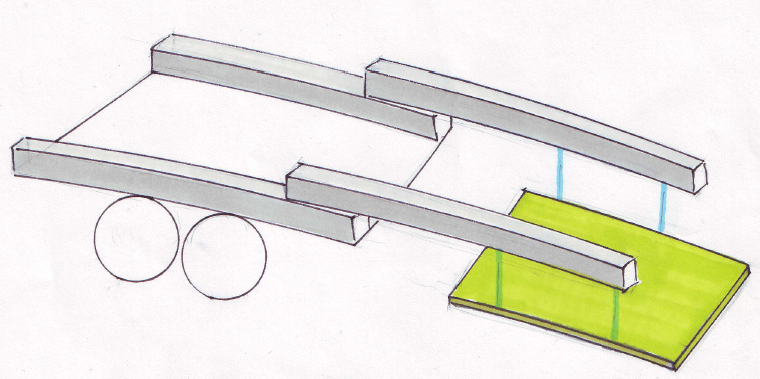
\includegraphics[width=0.6\textwidth]{images/Bildet_5}
\end{center}
\caption{Konsept 1}
\label{fig:Konsept 1}
\end{figure}

\subsubsection*{Konsept 2}
Satt sammen av følgende punkter fra Morfologisk tabell: 1.2 \& 1.4 - 2.1 - 3.2 - 4.1 - 5.3 - 6.4 - 7.4. I dette konseptet settes bilen først opp på en ramme som det er festet hjul under. Oppe på rammen skal undersiden av bilen hvile mot en pute, slik som på dagens løsning. Denne rammen skal så draes opp tilhengerdøren bak og inn i tilhengeren ved hjelp av en vaier som blir drevet av en manuell vinsj. Dette konseptet krever at hjulene på rammen er montert helt foran og bak slik at denne ikke tar nedi. Det må også monteres noen hjul på tilhengerkanten som rammen kan rulle på når den skal over kanten. Ellers vil den ta nedi også her.

\begin{figure}[H]
\begin{center}
\leavevmode
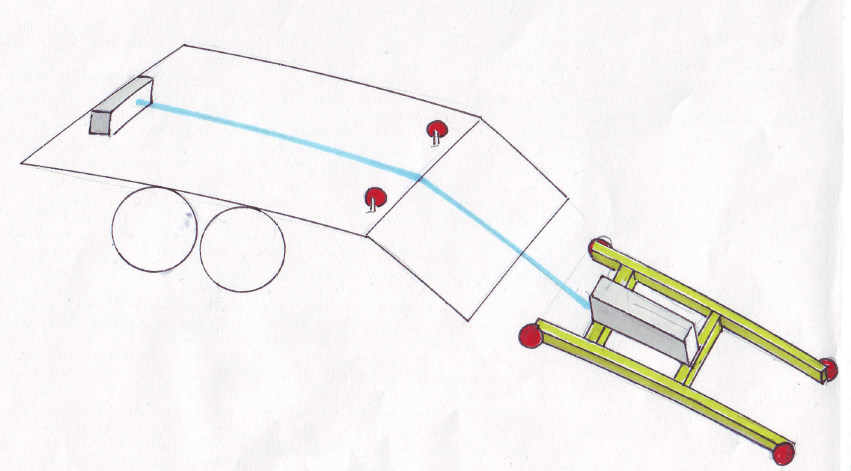
\includegraphics[width=0.6\textwidth]{images/Bildet_4}
\end{center}
\caption{Konsept 2}
\label{fig:Konsept 2}
\end{figure}

\subsubsection*{Konsept 3}
Satt sammen av følgende punkter fra Morfologisk tabell: 1.2 - 2.1 \& 2.2 - 3.2 - 4.6 - 5.3 - 6.4 - 7.4. I likhet med Konsept 2 settes bilen opp på en ramme slik at understellet hviler mot en pute. Under rammen er det montert hjul på samme måte som i Konsept 2. Rammen skyves opp tilhengerdøren bak og inn i tilhengeren ved hjelp av direkte manuell kraft.  Det monteres hjul på tilhengerkanten som rammen kan rulle på når den skal over denne. For å hindre at rammen skal ``tippe'' når bilen skal tas ut av tilhengeren og rammen kommer et stykke utover kanten på tilhengeren, skal det monteres en ``støttebrakett'' på hver side av rammen. Denne skal hindre at rammen tipper ned, inntil den har kommet en viss lengde ut av tilhengeren. På denne måten blir rammen enklere å kontrollere og sikkerheten ivaretas på en bedre måte.

\begin{figure}[H]
\begin{center}
\leavevmode
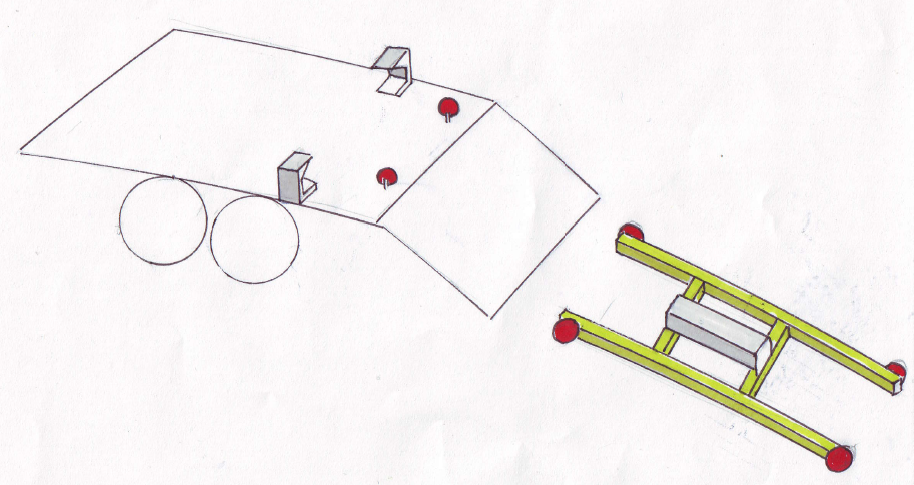
\includegraphics[width=0.6\textwidth]{images/Bildet_6}
\end{center}
\caption{Konsept 3}
\label{fig:Konsept 3}
\end{figure}

\subsection{Evaluering og valg av konsept}
Evaluerer de tre konseptene opp mot hverandre ved å sette de inn i en evalueringsmatrise. Ulike egenskaper blir vektet med poengsum fra 1 til 4, hvor en er dårligst og 4 er best. De ulike konseptene blir så gitt poeng fra 1 til 3 etter hvor gode de er på de ulike genskapene. 1 er dårligst og 3 er best. Til slutt blir vektingen av egenskapene addert med poengene og summert sammen. Det konseptet med høyest totalsum er det beste.

\begin{table}[H]
\begin{center}
\begin{tabular}{| l | c |c | c | c |}
\hline
\multicolumn{5}{|c|}{Evalueringsmatrise} \\
\hline
\textbf{Egenskap} & \textbf{Vekting} & Poeng Konsept 1 & Poeng Konsept 2 & Poeng Konsept 3\\
\hline
Lav kompleksitet & 2 & 1 & 3 & 3\\
\hline
Lav pris &4 & 1 & 2 & 2\\
\hline
Brukervennlighett & 4 & 3 & 1 & 2\\
\hline
Lav vekt & 3 & 1 & 3 & 3\\
\hline
Kvalitet & 4 & 3 & 2 & 2\\
\hline
Modifiserbar & 1 & 1 & 3 & 3\\
\hline
Funksjonalitet & 4 & 3 & 2 & 2\\
\hline
\multicolumn{2}{|l|}{Total poengsum} & 46 & 46 & 50 \\
\hline
\end{tabular}
\end{center}
\caption{Evealueringsmatrise}
\end{table}

\begin{flushleft}
Ser at Konsept 3 får høyest poengsum, det velges derfor å gå videre med dette konseptet.
\end{flushleft}

